% !TEX root = ../main.tex
\section{Experiments} \label{sec:experiments}


\subsection{Cauchy} \label{subsec:cauchy}

\begin{figure}[ht]
    \begin{subfigure}{\linewidth}
    \centering
    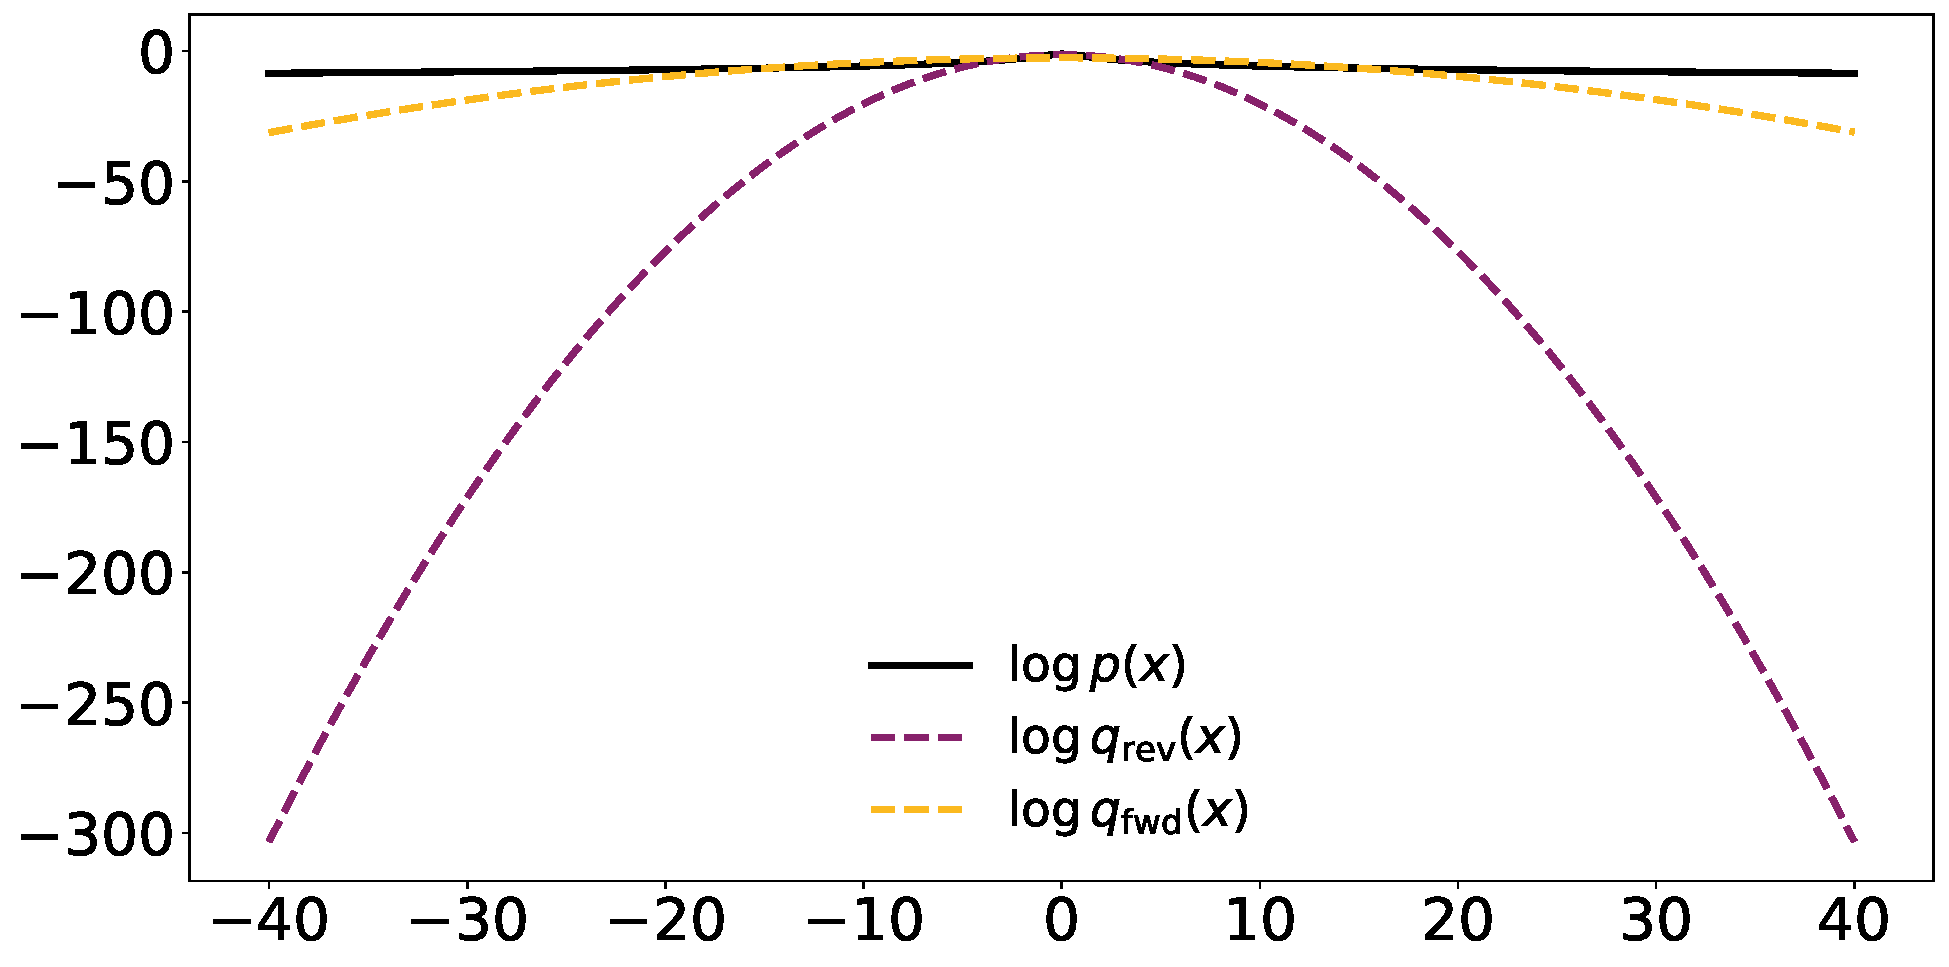
\includegraphics[width=0.8\linewidth]{fig/cauchy_logq.pdf}
    \caption{Log density}
    \label{fig:cauchy_lp}
    \end{subfigure}\\[1ex]
    \begin{subfigure}{\linewidth}
    \centering
    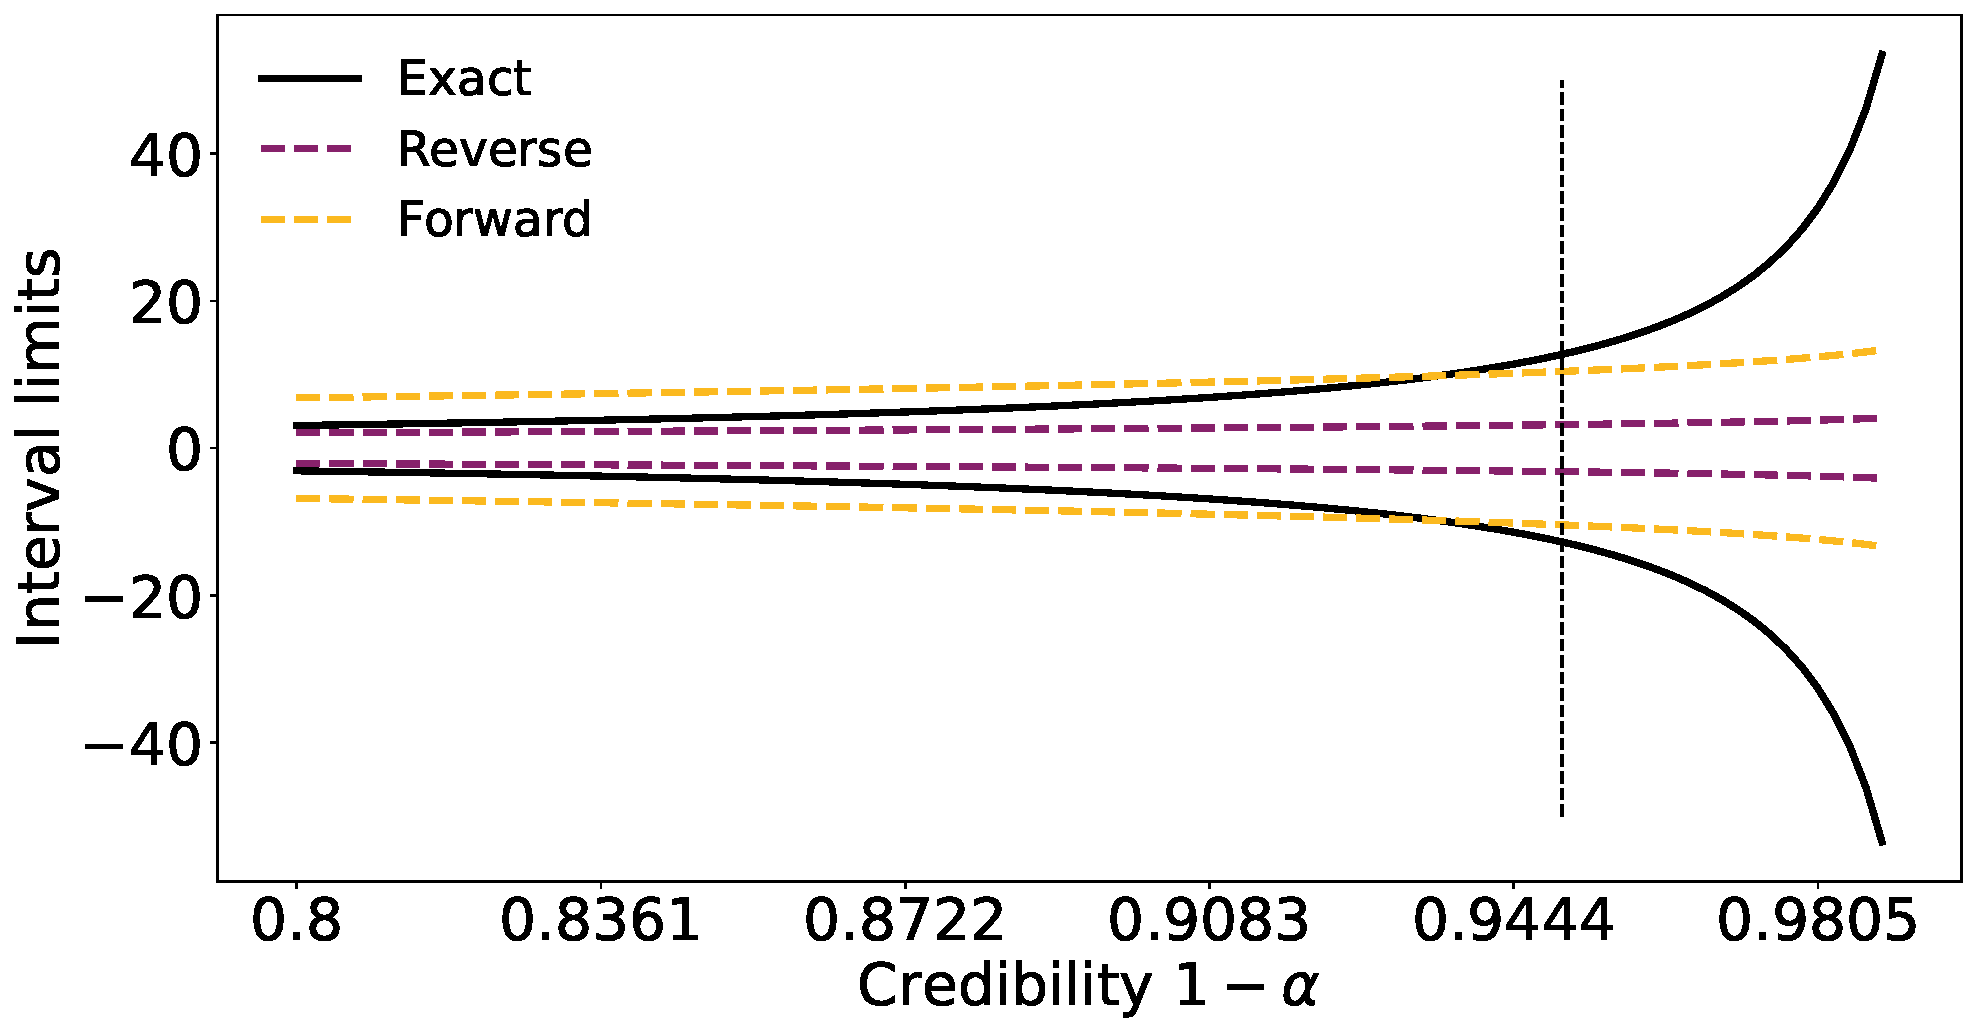
\includegraphics[width=0.8\linewidth]{fig/cauchy_cilims.pdf}
    \caption{CI limits}
    \label{fig:cauchy_lims}
    \end{subfigure}\\[1ex]
    \begin{subfigure}{\linewidth}
    \centering
    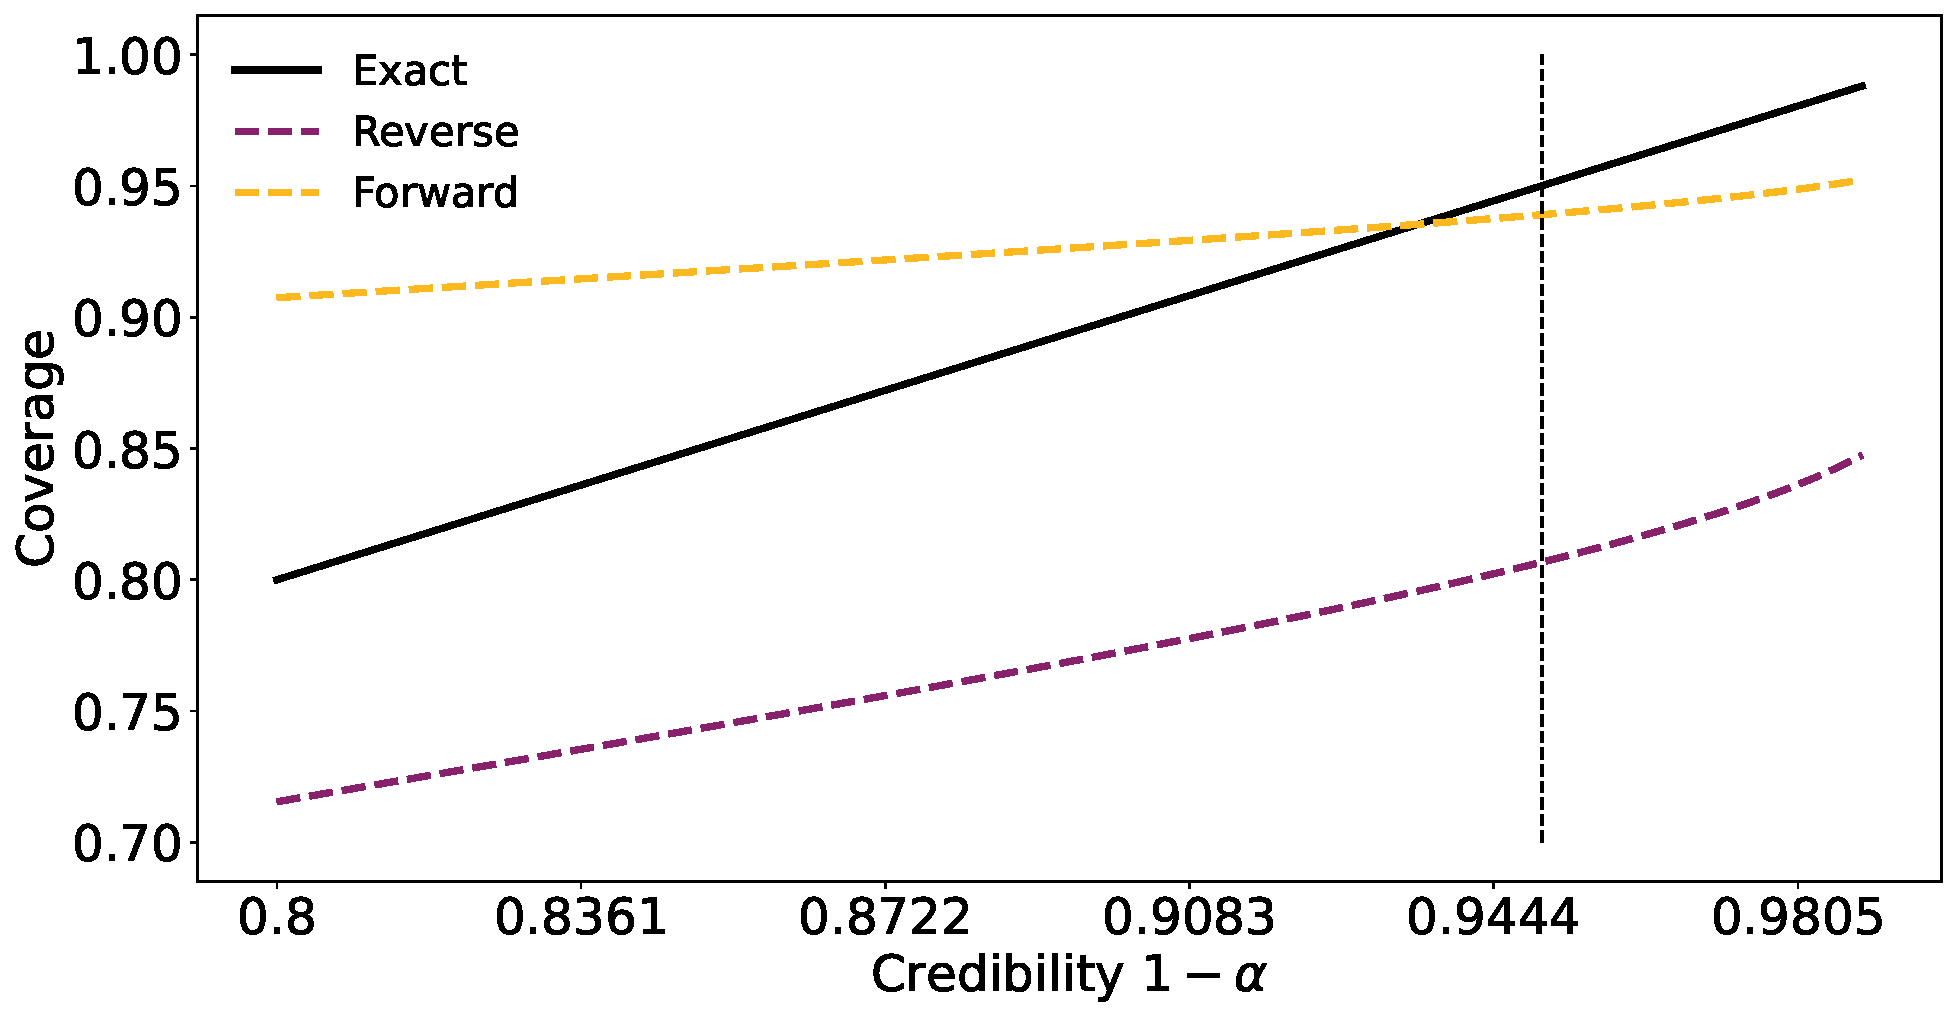
\includegraphics[width=0.8\linewidth]{fig/cauchy_cicoverage.pdf}
    \caption{CI coverage}
    \label{fig:cauchy_coverage}
    \end{subfigure}
    \caption{Results on the Cauchy distribution.}
    \label{fig:cauchy}
\end{figure}



\subsection{Logistics regression} \label{subsec:logreg}

\begin{figure}[ht]
    \begin{subfigure}{0.475\linewidth}
    \centering
    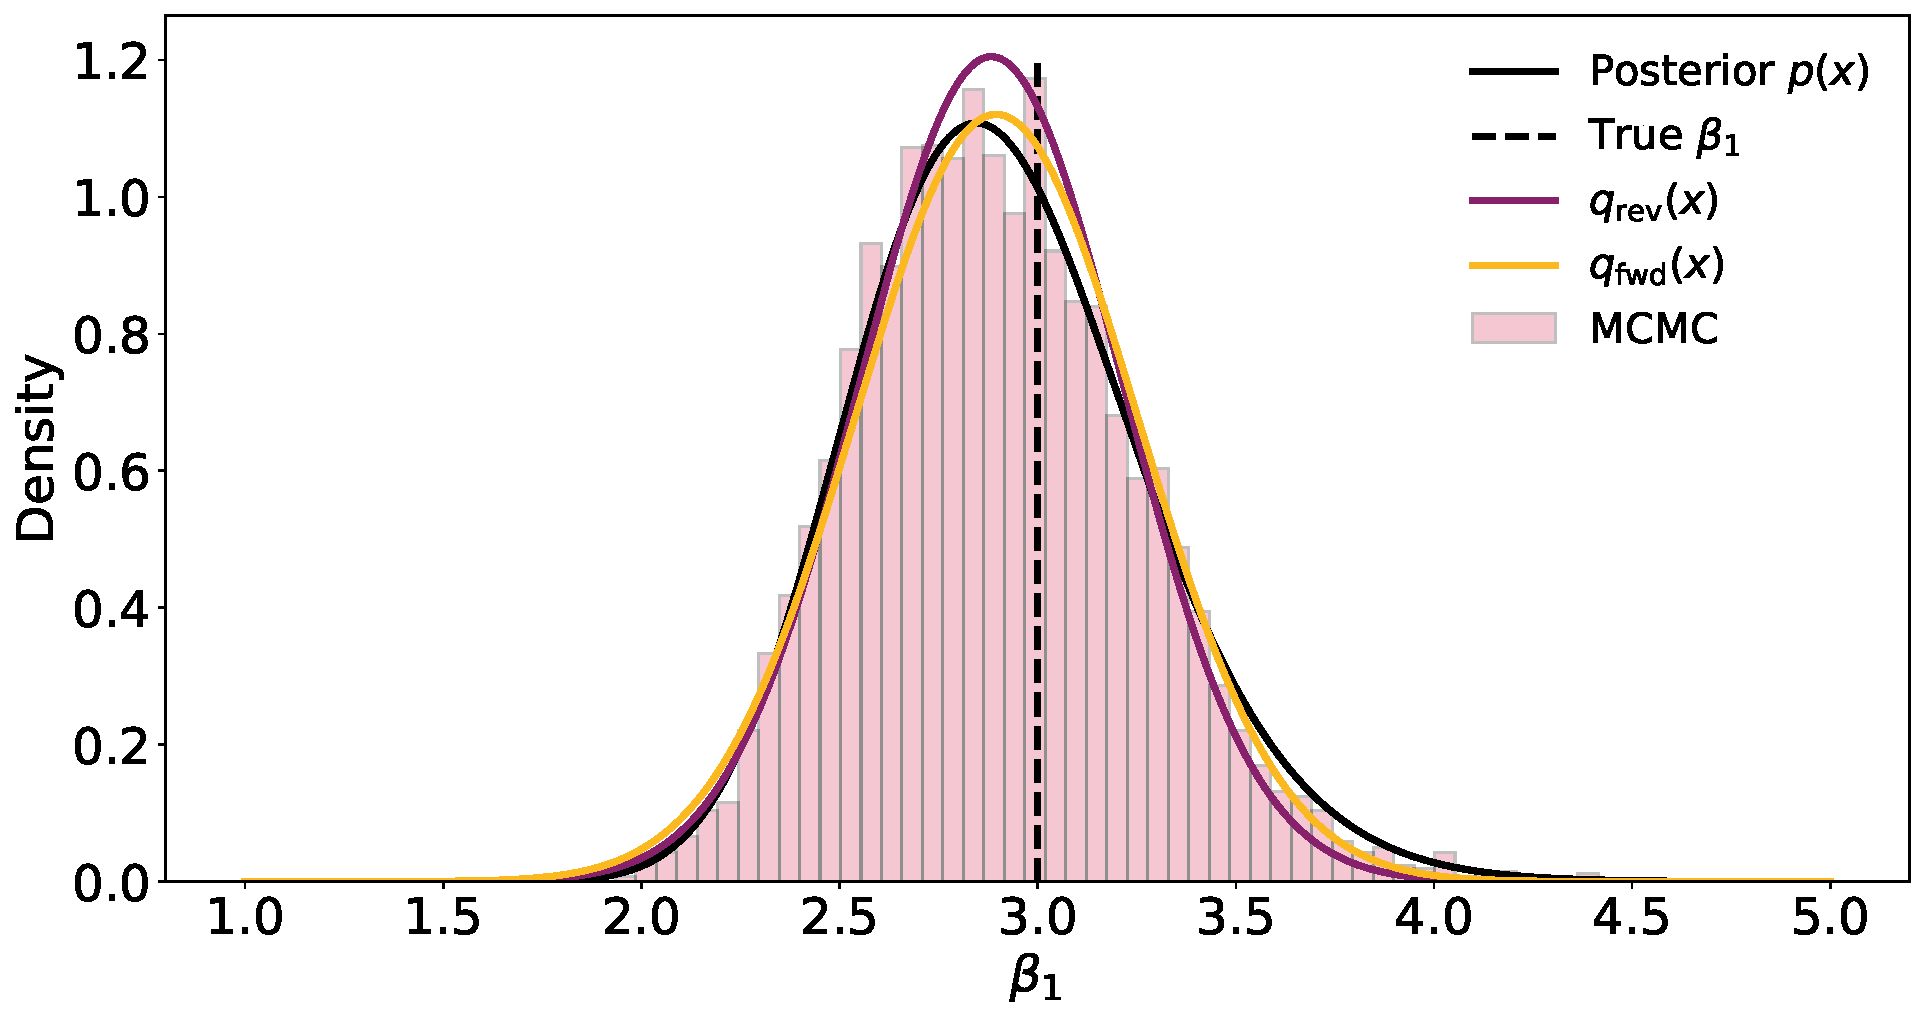
\includegraphics[width=\linewidth]{fig/logreg_q.pdf}
    \caption{Density}
    \label{fig:logreg_p}
    \end{subfigure}%
    \begin{subfigure}{0.475\linewidth}
        \centering
        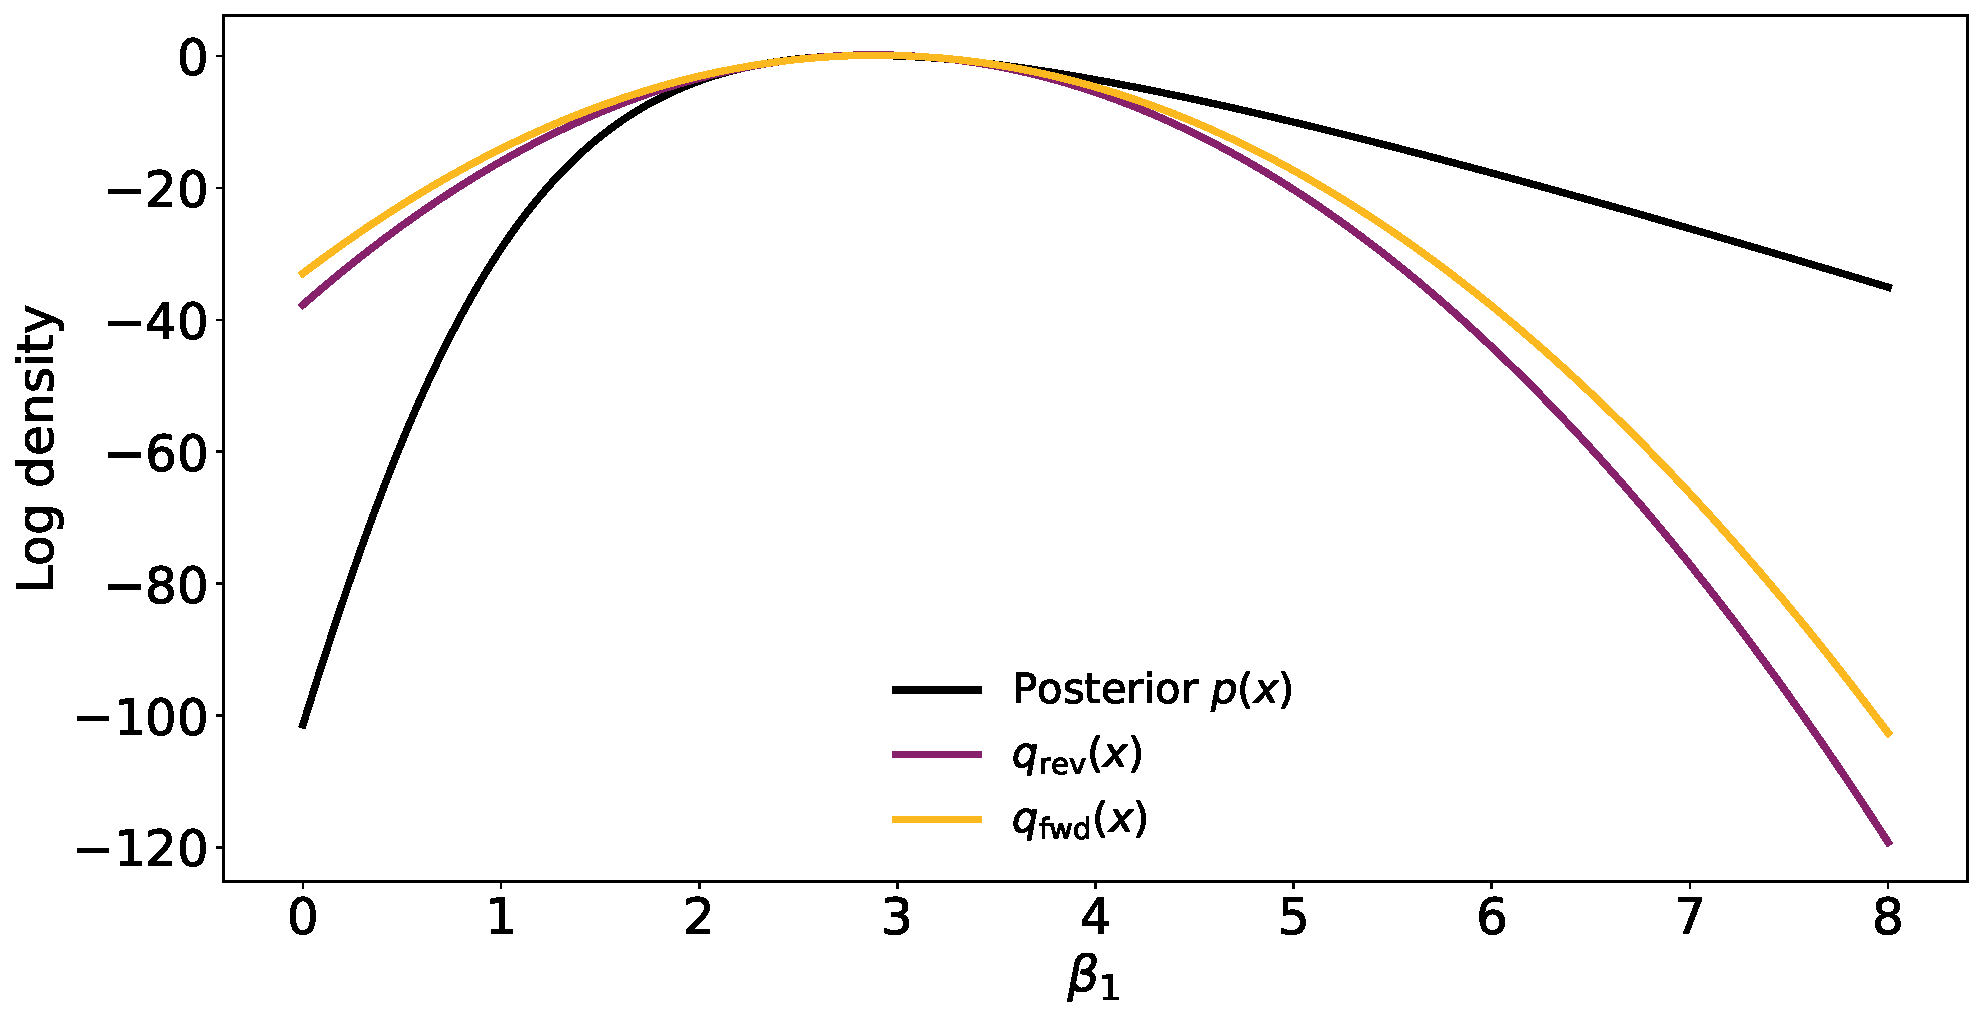
\includegraphics[width=\linewidth]{fig/logreg_logq.pdf}
        \caption{Log density}
        \label{fig:logreg_lp}
        \end{subfigure}\\[1ex]
    \begin{subfigure}{\linewidth}
    \centering
    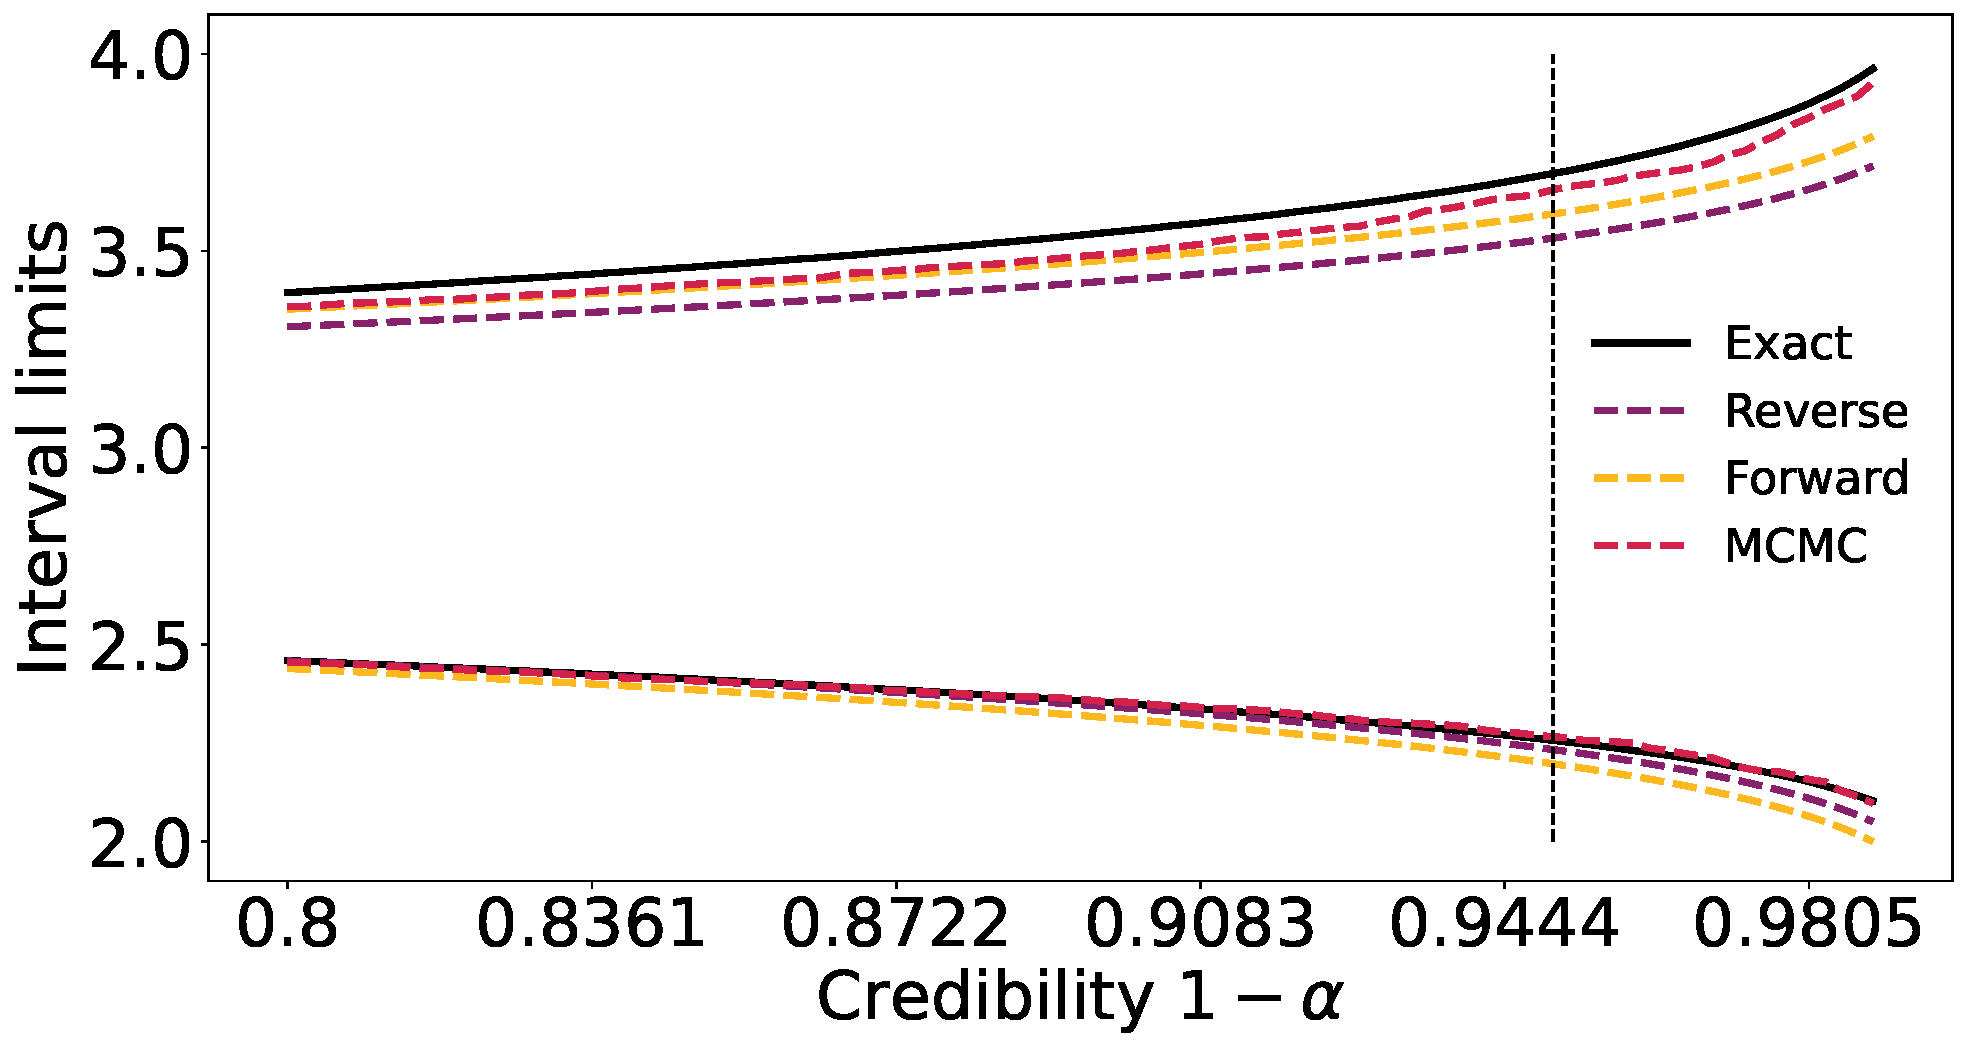
\includegraphics[width=0.8\linewidth]{fig/logreg_cilims.pdf}
    \caption{CI limits}
    \label{fig:logreg_lims}
    \end{subfigure}\\[1ex]
    \begin{subfigure}{\linewidth}
    \centering
    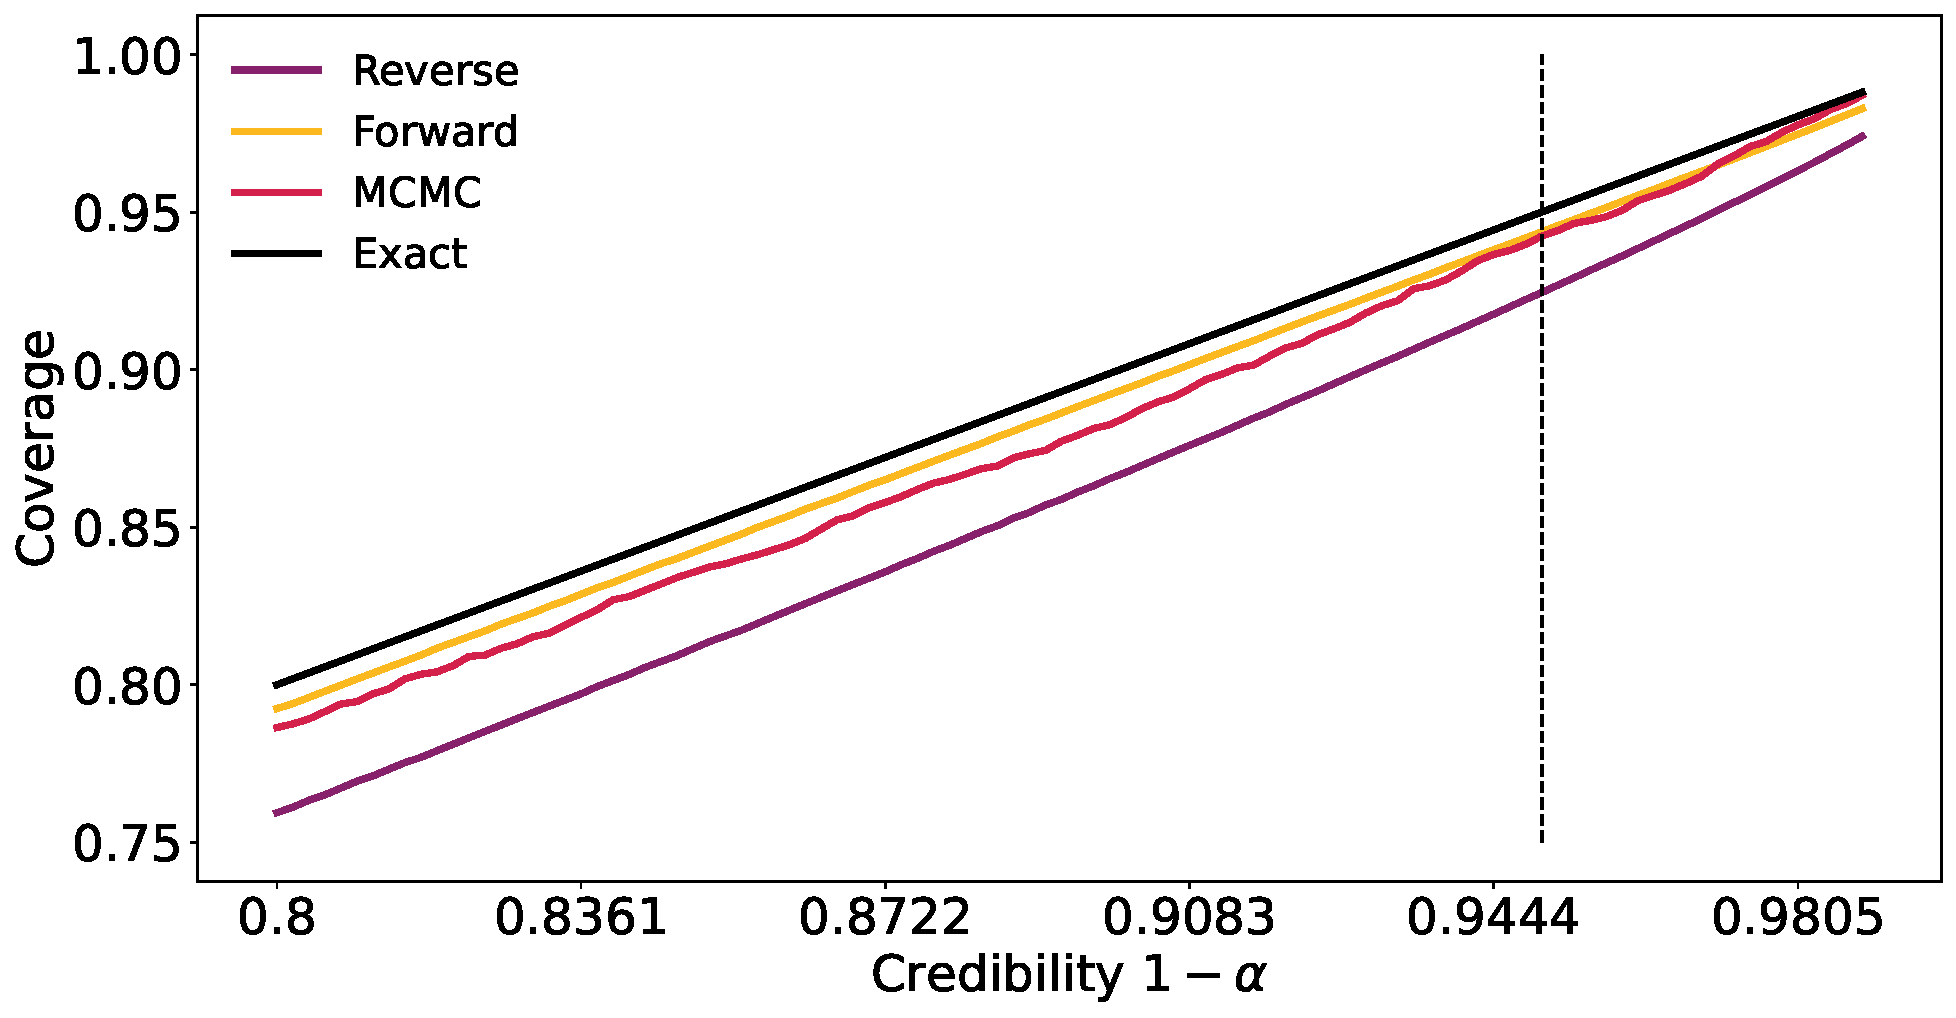
\includegraphics[width=0.8\linewidth]{fig/logreg_cicoverage.pdf}
    \caption{CI coverage}
    \label{fig:logreg_coverage}
    \end{subfigure}
    \caption{Results on the logistic regression example.}
    \label{fig:logreg}
\end{figure}
